A Transfer�ncia Eletr�nica Dispon�vel (TED) � uma transa��o financeira de valores entre diferentes bancos. Um economista decide analisar os valores enviados por meio de TEDs entre cinco bancos (1, 2, 3, 4 e 5) durante um m�s. Para isso, ele disp�e esses valores em uma matriz $A=[a_{ij}]$, em que $1 \leq i \leq 5$ e $1 \leq j \leq 5$, e o elemento $a_{ij}$ corresponde ao total proveniente das opera��es feitas via TED, em milh�o de real, transferidos do banco i para banco j durante o m�s. Observe que os elementos a .. = O, uma vez que TED � uma transfer�ncia entre bancos distintos. Esta � a matriz obtida para essa an�lise:

\begin{figure}[h]
\centering
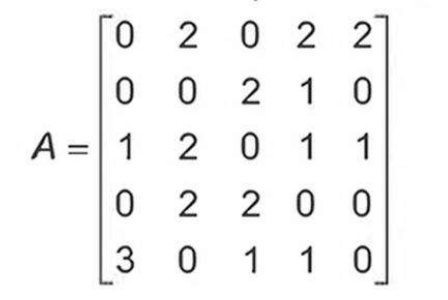
\includegraphics[width=8cm]{../figuras/q146-2018.png}
\end{figure}

Com base nessas informa��es, o banco que transferiu a maior quantia via TED � o banco 

\begin{enumerate}
\item[a)]1.
\item[b)]2.
\item[c)]3.
\item[d)]4.
\item[e)]5.
\end{enumerate}